\section{Backup slides}

\begin{slide}[toc=FT in MC generators]{Formation time in MC generators}
 
 \twocolumn
 {
 {\centering Formation time for nucleons\\}\mbox{}\\
 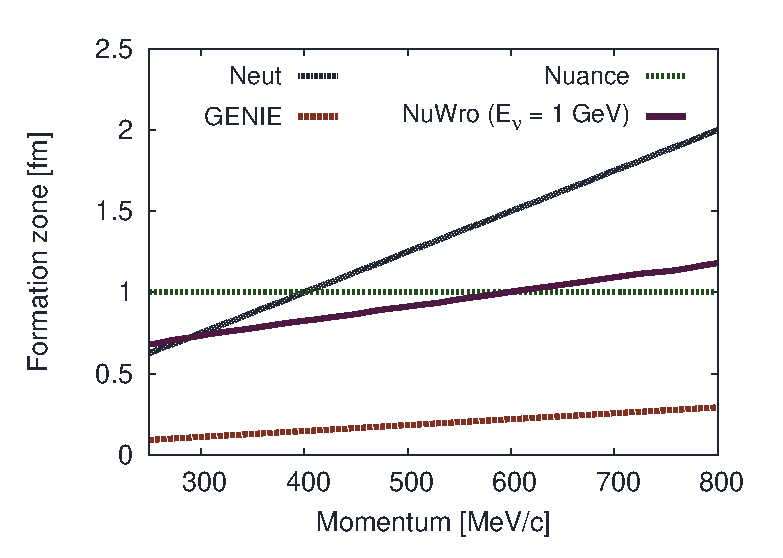
\includegraphics[width = \columnwidth]{img/fzn.eps}
 }
 {
 {\centering Formation time for pions\\}\mbox{}\\
 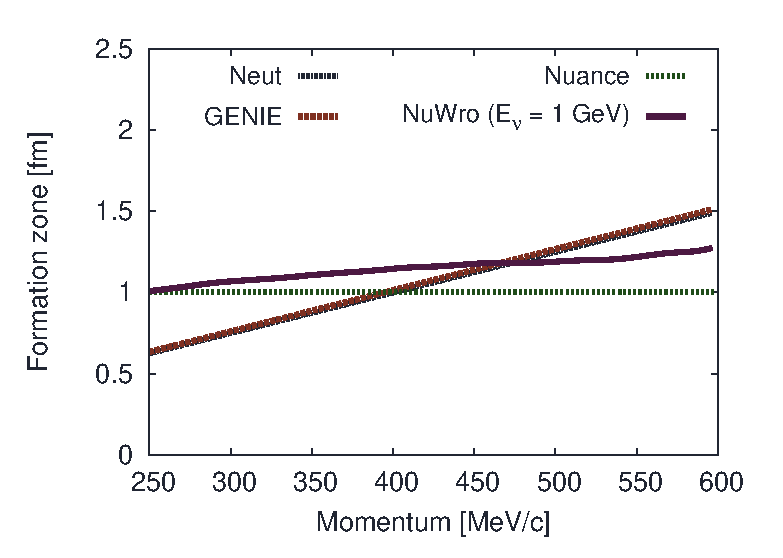
\includegraphics[width = \columnwidth]{img/fzp.eps} 
 }
 
 \begin{itemize}
 
  \item NUANCE uses constant formation length $x = 1$~fm.
  
  \item NEUT uses SKAT parametrization ($\mu^2 = 0.08 \pm 0.04\mbox{ GeV}^2$): \vspace{-5pt}$$x = \frac{|\vec p|}{\mu^2}$$\vspace{-25pt}
 
  \item GENIE uses Rantf  parametrization (assuming transverse momentum $p_T = 0$): \vspace{-15pt}$$x = \tau_0 \frac{E}{M} = \tau_0 \gamma$$
  
 \end{itemize}
 
\end{slide}

\begin{slide}{Form factors}
 \vspace{-10pt}
 \onslide*{1}
 {
    $$\Gamma^\mu_{CC}(q) = \gamma^\mu {\color{pdcolor4}F_1^V (Q^2)} + \frac{i\sigma^{\mu\nu}q_\nu}{2M} {\color{pdcolor4}F_2^V (Q^2)} - \gamma^\mu\gamma_5 {\color{pdcolor5}G_A (Q^2)} - q^\mu\gamma_5 \frac{{\color{pdcolor6}F_P(Q^2)}}{2M}$$
    
    \begin{itemize}
     
     \item Vector form factors are expressed by electromagnetic form factors {\it(Conserved Vector Current - CVC)}: 
     
     $${\color{pdcolor4}F_{1,2}^V(Q^2)} = F_{1,2}^p(Q^2) - F_{1,2}^n(Q^2)$$
     
     \item Axial form factor is assumed to have a dipole form:
     
     $${\color{pdcolor5}G_A(Q^2)} = \frac{g_A}{\left(1 + Q^2/M_A^2\right)^2}$$
     
     \item Pseudoscalar form factor is related to the axial one {\it(Partially Conserved Axial Current - PCAC)}:
     
     $${\color{pdcolor6}F_P(Q^2)} = \frac{4M^2}{m_\pi^2 + Q^2}G_A(Q^2)$$
     
    \end{itemize}
 }
 \onslide*{2}
 {
 $$\hspace{-10pt}\Gamma^\mu_{NC, p(n)} = \gamma^\mu {\color{pdcolor4}F_1^{NC, p(n)} (Q^2)} + \frac{i\sigma^{\mu\nu}q_\nu}{2M} {\color{pdcolor4}F_2^{NC, p(n)} (Q^2)} - \gamma^\mu\gamma_5 {\color{pdcolor5}G_A^{NC, p(n)} (Q^2)}$$
 
 \begin{itemize}
  
     \item Vector form factors are expressed by electromagnetic form factors {\it(Conserved Vector Current - CVC)}: 
     {\footnotesize\vspace{10pt}
     $$\hspace{-20pt}{\color{pdcolor4}F_{1,2}^{NC, p(n)}(Q^2)} = \pm\frac{1}{2}\left(F_{1,2}^p(Q^2) - F_{1,2}^n(Q^2)\right) - 2\sin^2\theta_WF_{1,2}^{p(n)}(Q^2) - \frac{1}{2}F_{1,2}^s(Q^2)$$
     }
     \item Axial form factor is assumed to have a dipole form:
     
     $${\color{pdcolor5}G_A^{NC,p(n)}(Q^2)} = \pm\frac{1}{2}G_A(Q^2) - \frac{1}{2}{\color{pdcolor6}G_A^s(Q^2)}$$
 
    \item The axial strange form factor is assumed to have a dipole form:
    
     $${\color{pdcolor6}G_A^s(Q^2)} = \frac{g_A^s}{\left(1 + Q^2/M_A^2\right)^2}$$
     
 \end{itemize}
 }

 
\end{slide}

\begin{slide}[toc= TE model]{Transverse Enhancement model}
 
 \begin{itemize}
  
  \vspace{10pt}
  \item In the Transverse Enhancement model the two body current contribution is introduced by the modification of the vector magnetic form factors:
  
  $$G^{p,n}_M \rightarrow \tilde G^{p,n}_M = \sqrt{1 + AQ^2\exp{\left(-\frac{Q^2}{B}\right)}}G^{p,n}_M(Q^2)$$
  
  \item $A, B$ are established from the electron data.
  
  \item The cross section for $np-nh$ can be obtained by taking the difference:
  
  $$\frac{\mbox{d}^2\sigma^{np-nh}}{\mbox{d}q\mbox{d}\omega} \equiv \frac{\mbox{d}^2\sigma^{QEL}}{\mbox{d}q\mbox{d}\omega}(\tilde G^{p,n}_M) - \frac{\mbox{d}^2\sigma^{QEL}}{\mbox{d}q\mbox{d}\omega}(G^{p,n}_M)$$
  
  \item The disadvantage of the model is lepton kinematics (``copied'' from the QEL scattering).
 
 \end{itemize}
 
\end{slide}
